\chapter{O vigia da direção}\label{cap:direcao}

O capítulo da memória terminou com uma pergunta que ele mesmo abriu: apagar os dias apaga, com eles,
a ordem em que vieram, e é a ordem que diz para onde o tempo aponta. Falta medir se essa direção pode
ser \textbf{vigiada}, e vigiada com garantia.

\section{O orçamento que a conta promete}

O instrumento é o mesmo das outras travessias: uma estatística, um limiar e um orçamento declarado. A
estatística é o terceiro momento do incremento, e a razão de ser dele está na proposição abaixo.

\begin{proposicao}[o desvio do nulo]\label{prop:nulo-da-direcao}
Se os incrementos de um mundo forem simétricos e de escala constante, a média do cubo do incremento
padronizado tem média zero e desvio $\sqrt{15/n}$ numa janela de $n$ dias.
\end{proposicao}

\begin{proof}
Para um normal padrão $z$, $E[z^3] = 0$ pela simetria, e $E[z^6] = 15$. O cubo tem, então, média
zero e variância $15$; a média de $n$ deles tem variância $15/n$, e a raiz disso é o desvio.
\end{proof}

Com a janela de \numDirecaoJanela{} dias, o \cref{prop:nulo-da-direcao} dá \numDirecaoConta{}, e o limiar de
\numDirecaoZ{} desvios fica em \numDirecaoLimiar{}. A conta promete, com esse limiar,
\numDirecaoContaTaxa{} alarmes por bloco num mundo sem direção nenhuma.

O primeiro fracasso do capítulo é o que acontece quando se acredita nessa promessa. Medindo o mundo
simétrico --- \numDirecaoSementes{} mundos sorteados, \numDirecaoBlocosPorMundo{} janelas cada e a
primeira gasta para padronizar, \numDirecaoBlocosNulo{} blocos medidos ---, a dispersão da
estatística é de \numDirecaoNuloDispersao{} em vez dos \numDirecaoConta{} da conta, e a taxa de
alarme é de \numDirecaoNuloTaxa{} por bloco: \numDirecaoRazaoDasTaxas{} vezes o prometido. O limiar
que entrega a promessa é \numDirecaoLimiarMedido{}, contra \numDirecaoLimiar{} da conta --- um terço mais
alto, \numDirecaoLimiarMedidoRazao{} vezes. A média do nulo, medida, é \numDirecaoNuloMedia{}, que é zero
dentro do ruído --- o que está errado na conta é a dispersão, e não o centro.

O motivo da diferença não é um erro de conta. A conta supõe escala constante, e o mundo deste livro
tem agrupamento: num bloco em que a oscilação se agita, os incrementos padronizados ficam longe do
normal, e o cubo deles cresce mais depressa do que a conta prevê.

\section{O instrumento, conferido}

Antes de usar o instrumento sobre o dado, é preciso saber que ele mede o que diz medir. A conferência
é inverter o relógio: se a estatística não trocar de sinal quando o filme roda ao contrário, ela não
está medindo direção nenhuma.

Aplicada às três séries deste livro, a conferência passa exatamente. O terceiro momento dos
incrementos é \numDirecaoIndiceMomento{} no índice, \numDirecaoIbovespaMomento{} no Ibovespa e
\numDirecaoBitcoinMomento{} no Bitcoin; invertidas as três séries, os três números trocam de sinal
sem trocar de tamanho, indo a \numDirecaoIndiceInvertida{}, \numDirecaoIbovespaInvertida{} e
\numDirecaoBitcoinInvertida. Em desvios da conta do nulo, a direção do índice vale
\numDirecaoIndiceRazao{} desvios em \numDirecaoIndiceDias{} dias, e a do Ibovespa
\numDirecaoIbovespaRazao{}.

Os três mercados têm, então, direção, e ela é grande: \numDirecaoBitcoinRazao{} desvios no Bitcoin, que
entra na conta com \numDirecaoBitcoinDias{} dias, em \numDirecaoBitcoinBlocos{} blocos de um ano, contra
\numDirecaoIbovespaDias{} dias e \numDirecaoIbovespaBlocos{} blocos do Ibovespa.
O que falta é a segunda metade da promessa --- quanto tempo um vigia leva para vê-la enquanto o mundo
corre.

\section{Quanto tempo para ver}

O vigia lê a estatística em blocos e decide ao fim de cada bloco. A tabela dá o que ele vê, para
mundos com direção declarada, nos dois limiares.

\begin{table}[htbp]
  \centering
  \small
  \begin{tabular}{rrrr}
    \hline
    direção do & estatística & acerto no & acerto no \\
    mundo & medida & limiar da conta & limiar honesto \\
    \hline
    \numDirecaoAssimetriaSimetrico & \numDirecaoEstatisticaSimetrico & \numDirecaoAcertoSimetrico & \numDirecaoAcertoHonestoSimetrico \\
    \numDirecaoAssimetriaDoisCentesimos & \numDirecaoEstatisticaDoisCentesimos & \numDirecaoAcertoDoisCentesimos & \numDirecaoAcertoHonestoDoisCentesimos \\
    \numDirecaoAssimetriaCincoCentesimos & \numDirecaoEstatisticaCincoCentesimos & \numDirecaoAcertoCincoCentesimos & \numDirecaoAcertoHonestoCincoCentesimos \\
    \numDirecaoAssimetriaDezCentesimos & \numDirecaoEstatisticaDezCentesimos & \numDirecaoAcertoDezCentesimos & \numDirecaoAcertoHonestoDezCentesimos \\
    \numDirecaoAssimetriaVinteCentesimos & \numDirecaoEstatisticaVinteCentesimos & \numDirecaoAcertoVinteCentesimos & \numDirecaoAcertoHonestoVinteCentesimos \\
    \numDirecaoAssimetriaQuarentaCentesimos & \numDirecaoEstatisticaQuarentaCentesimos & \numDirecaoAcertoQuarentaCentesimos & \numDirecaoAcertoHonestoQuarentaCentesimos \\
    \hline
  \end{tabular}
  \caption{O acerto do vigia da direção em mundos com assimetria declarada, com o limiar da conta e
    com o limiar honesto. A primeira linha é o mundo sem direção: ali o acerto é o gasto em alarme
    falso, e é contra ele que as outras linhas se leem.}
  \label{tab:direcao}
\end{table}

A leitura é dura com a promessa. Uma direção de \numDirecaoAssimetriaCincoCentesimos{} --- que já é
uma direção declarada, posta de propósito no mundo --- é vista em
\numDirecaoAcertoHonestoCincoCentesimos{} dos blocos. O índice americano tem direção de
\numDirecaoIndiceMomento{}, um sexto acima disso --- mais forte que o mundo declarado, e longe do dobro. E a primeira linha mostra o preço: no mundo sem
direção nenhuma, o vigia ainda gasta \numDirecaoAcertoHonestoSimetrico{} dos seus blocos em alarme
falso, e é esse o piso contra o qual qualquer acerto tem de ser lido.

A dispersão da estatística sobe junto com a direção do mundo: ela vai de
\numDirecaoDispersaoSimetrico{} no mundo sem direção a \numDirecaoDispersaoQuarentaCentesimos{} no mais
assimétrico, passando por \numDirecaoDispersaoDoisCentesimos{},
\numDirecaoDispersaoCincoCentesimos{}, \numDirecaoDispersaoDezCentesimos{} e
\numDirecaoDispersaoVinteCentesimos{}. Um mundo com direção é também um mundo mais difícil de ler, e as
duas coisas não se separam: a mesma assimetria que o vigia procura é a que embaralha a estatística.

\begin{figure}[htbp]
  \centering
  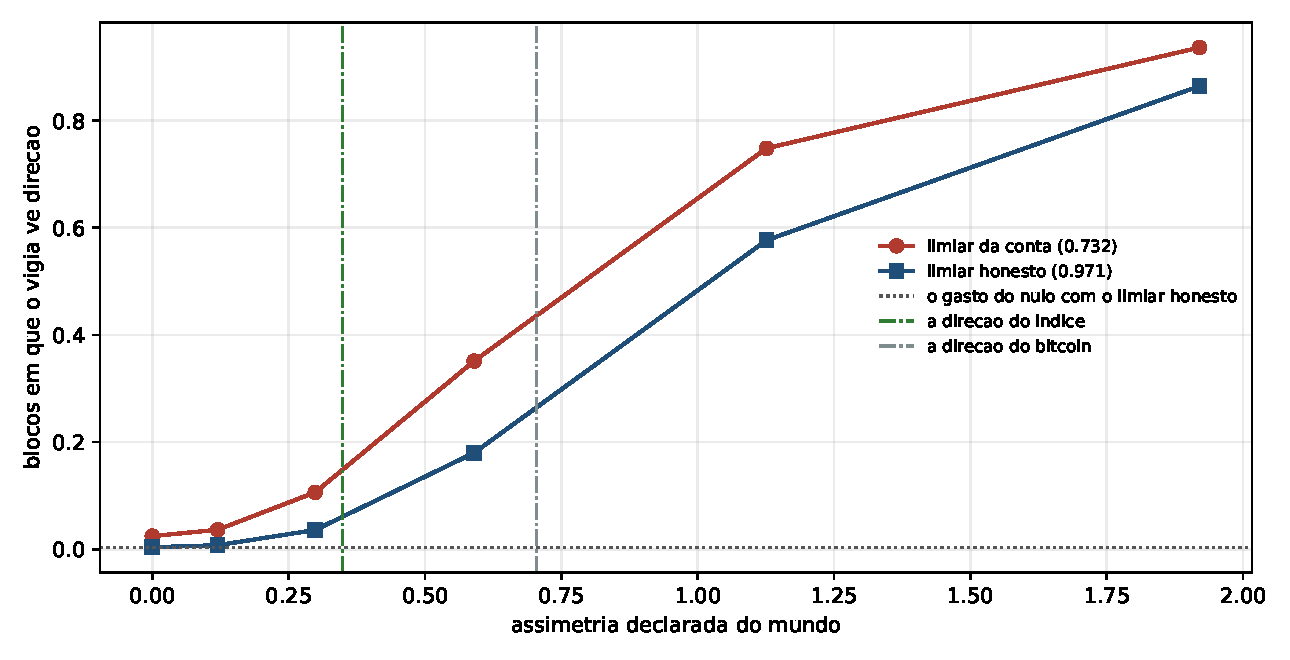
\includegraphics[width=\linewidth]{figuras/E13_vigia_da_direcao_2.pdf}
  \caption{O acerto do vigia contra a direção declarada do mundo, nos dois limiares. As linhas
    verticais marcam a direção medida no índice e no Bitcoin, e a linha pontilhada é o que o vigia
    gasta à toa com o limiar honesto.}
  \label{fig:acerto}
\end{figure}

\section{O ano não é a direção}

Falta o controle que separa o que é do vigia do que é do mundo. No dado real, a estatística de um bloco de um ano
é muito mais dispersa do que num mundo simétrico: \numDirecaoIndiceDispersaoBlocos{} no índice,
\numDirecaoIbovespaDispersaoBlocos{} no Ibovespa e \numDirecaoBitcoinDispersaoBlocos{} no Bitcoin,
contra \numDirecaoNuloDispersao{} lá. O vigia de bloco de um ano mede, então, o \textbf{caráter do ano} ---
e a seta do tempo aparece só quando se somam muitos anos.

\begin{figure}[htbp]
  \centering
  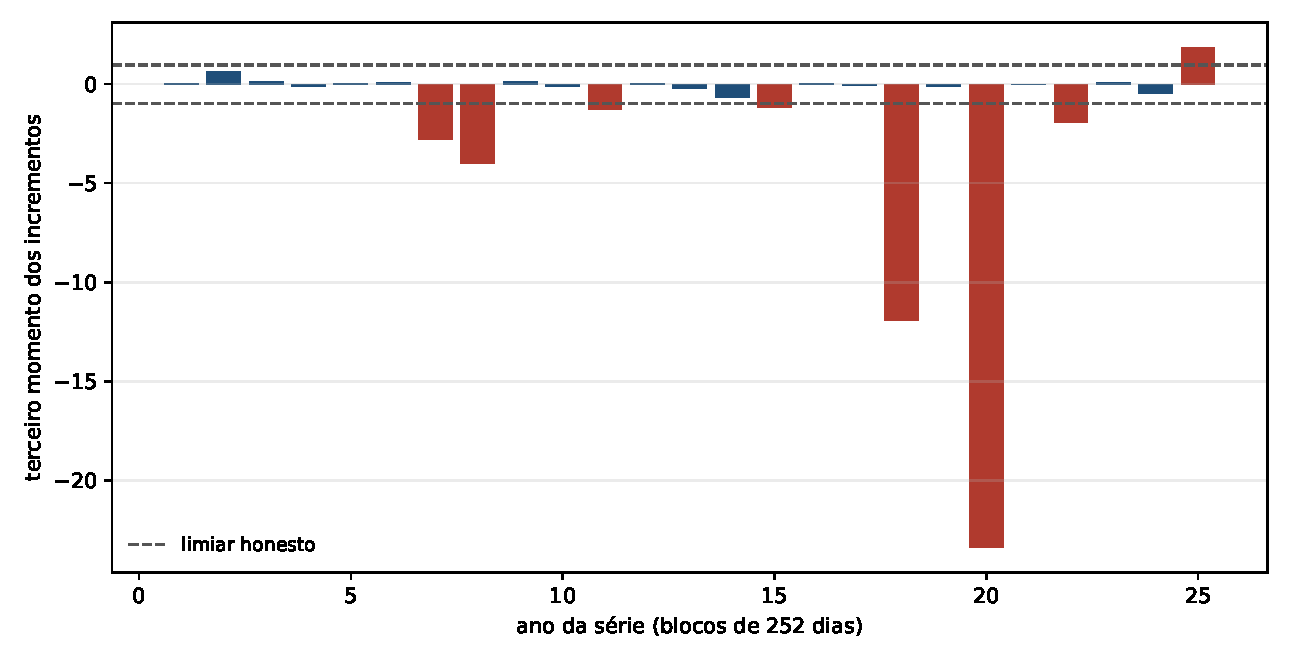
\includegraphics[width=\linewidth]{figuras/E13_vigia_da_direcao_1.pdf}
  \caption{O terceiro momento dos incrementos, ano a ano, no índice americano, com o limiar honesto.
    As barras em vermelho são os anos em que o vigia alarmaria.}
  \label{fig:anos}
\end{figure}

A figura mostra a consequência. Dos \numDirecaoIndiceBlocos{} anos do índice,
\numDirecaoIndiceBlocosAcima{} passam do limiar honesto, o que é
\numDirecaoIndiceAcertoHonesto{} dos anos, contra \numDirecaoIbovespaAcertoHonesto{} no Ibovespa e
\numDirecaoBitcoinAcertoHonesto{} no Bitcoin --- e
dois deles são os anos de quebra, o de dois mil e oito e o de dois mil e vinte; a dispersão de
\numDirecaoIndiceDispersaoBlocos{} vem sobretudo dos blocos de dois mil e dezoito e de dois mil e
vinte. Um vigia que decide ao fim de cada ano mede se aquele ano teve um tombo, e a seta do tempo fica para
depois.

\section{O que fica}

Fica a resposta da travessia, e ela tem duas partes que não podem ser separadas. A direção do tempo
existe no dado e é grande: \numDirecaoIndiceRazao{} desvios no índice, \numDirecaoBitcoinRazao{} no
Bitcoin, e o instrumento a confere trocando de sinal quando o relógio é invertido. E o vigia que
decide enquanto o mundo corre paga caro pela pressa: com o orçamento declarado, uma direção do tamanho
da que os mercados têm é vista em uma fração pequena dos anos, e nos outros o que ele encontra é o
caráter do ano.

Fica também o orçamento lido da medição. É a terceira vez nesta espiral que ele aparece: a conta
gaussiana prometeu \numDirecaoContaTaxa{} alarmes por bloco e o mundo simétrico entregou
\numDirecaoNuloTaxa{}, dez vezes mais. Quem calibrasse o vigia pela álgebra teria um vigia falador, e
acharia que o mundo tem direção onde só há agrupamento.

O fracasso seguinte é do mesmo objeto, medido noutra direção. Tudo o que este capítulo mediu foi a
direção de \textbf{uma} série. Quando as coisas ruins vêm juntas, há uma segunda pergunta de direção, e ela é sobre outra
coisa: numa queda conjunta, alguém cai primeiro. Se essa ordem se
repete, a perda conjunta também tem uma seta --- e é essa a última travessia que falta.
